\section{Tests}
\label{sec:tests}
In this section, we present a series of simulation results that try to answer to the following question: what improvement can we get in terms of fall prevention by using the robust controller?
We tested the proposed controller on a typical humanoid tasks (i.e. whole-body reaching) with the 30-degree-of-freedom humanoid robot HRP-2.
We carried out several batches of tests, each batch differing for the simulated uncertainties. 
Each batch was composed by 100 tests, which is not enough for being a statistically significant sampling, but was dictated by the computation time of our simulation environment (about 6 hours for 100 tests).
Each test consisted in trying to perform the reaching motion with the two controllers (classic and robust) until the robot either fell or reached the end of the motion.
The inertial parameter errors changed at each test, but they were the same for the two controllers.
We then measured the number of times each controller drove the robot to a fall and the average distance between the final end-effector position and the desired target.

\subsection{Simulation Environment}
\begin{table}[!tbp] 
\caption{Simulation parameters.}
\centering 
\begin{tabular}{p{1.1cm} | p{3.8cm} p{1.8cm}}
\hline 
	Symbol		& Meaning 				& Value \\ \rowcolor[gray]{.9}
\hline 
	$\dt$			& Simulation time step 		& 0.002 s \\
	$\dot{v}_j^{max}$ & Max joint acceleration		& $10 \, \text{rad} \, \text{s}^{-2}$ \\ \rowcolor[gray]{.9}
	$v_j^{max}$	& Max joint velocity			& $9.14 \, \text{rad} \, \text{s}^{-1}$ \\
	$\mu$		& Force friction coefficient		& 0.3 \\  \rowcolor[gray]{.9}
	$w_{reach}$	& Reaching weight 		& $1$ \\ 
	$w_{post}$ 	& Posture weight 			& $10^{-2}$ \\ \rowcolor[gray]{.9}
	$w_{force}$ & Force minimization weight 			& $10^{-5}$ \\ 
%	$K_p^{reach}$ 	& Reaching proportional gain 	& $20-80$ \\ \rowcolor[gray]{.9}
%	$K_p^{post}$ 	& Posture proportional gain 	& $20$ \\
[0.5ex] \hline 
\end{tabular} 
\label{table:simu_params} %\bigskip
\end{table}
To assess the proposed controller we developed a dedicated simulation environment based on a state-of-the-art algorithm for frictional contacts in multibody systems~\cite{Kaufman2008}. 
We integrated the equations of motion of the system with a first-order Euler scheme with fixed time step $\dt$.
Our choice of not using an off-the-shelf simulator is motivated by our desire to completely understand and control the simulation environment. 
The inertial parameters (masses and centers of mass) of the model used by the controller did not match those of the model used by the simulator. 
The random inertial-parameter errors were generated using uniform distribution. 
For masses, the maximum error was expressed in terms of percentage of the real values. 
For centers of mass, the maximum error was instead expressed in meters. 
In each test we specify which uncertainties were simulated. 
Table~\ref{table:simu_params} lists all the simulation and controller parameters.

\subsection{Task Description}
The control objective was defined by three tasks that the robot had to perform at the same time. 
Since the tasks are in conflict, we weighted them with hand-tuned parameters, according to their importance.
The three tasks, in order of decreasing priority, are:
\begin{itemize}
\item reach the desired target with the right end-effector (weight $w_{reach}$)
\item maintain initial joint posture (weight $w_{post}$)
\item minimize contact moments and tangential forces~\cite{Righetti2013} (weight $w_{force}$)
\end{itemize}


We carried out two sets of simulations.
In both cases HRP-2 executed a reaching motion that made its capture point reach the boundaries of its support polygon. 


\begin{figure*}[!tbph]
\centering
\begin{subfigure}
[Classic control illustrating the robot's loss of balance when the real capture point gets out of the support polygon]{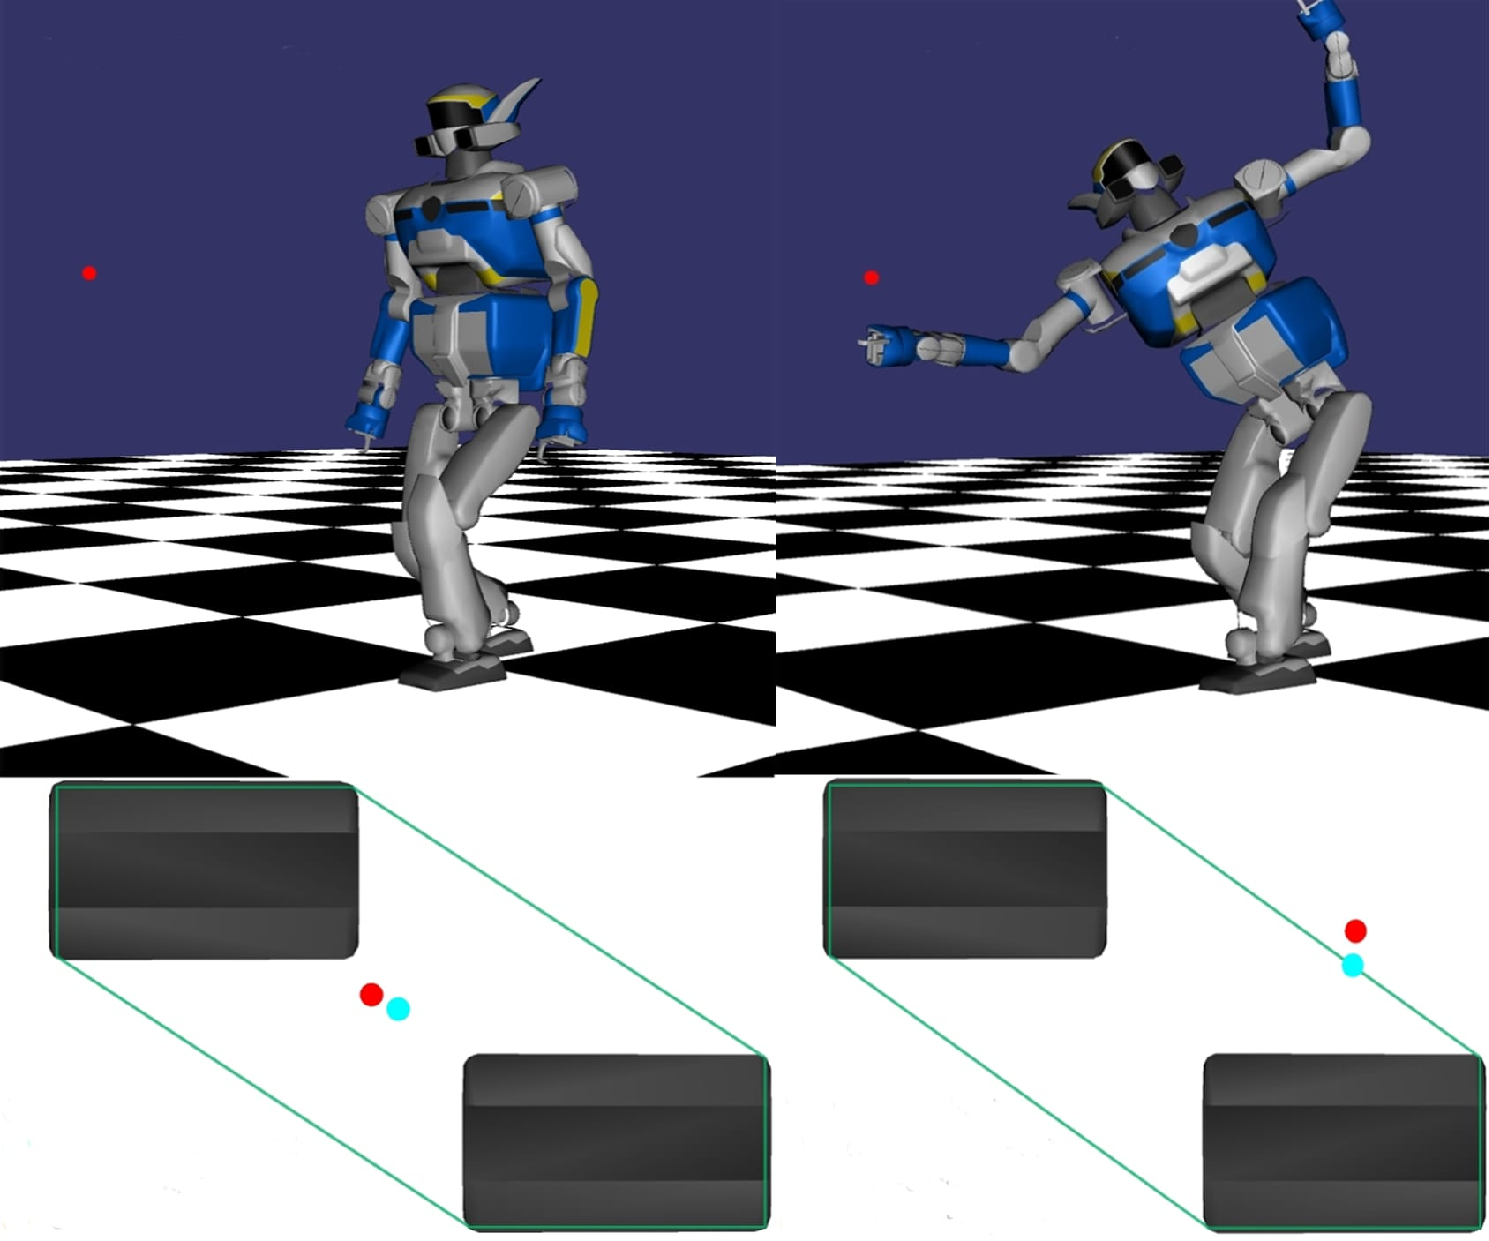
\includegraphics[scale=0.4]{rc_inertial_params/classic_merge.pdf}}\quad
\end{subfigure}
\begin{subfigure}
[Robust control illustrating the robot right end effector reaching close to the goal without losing balance]{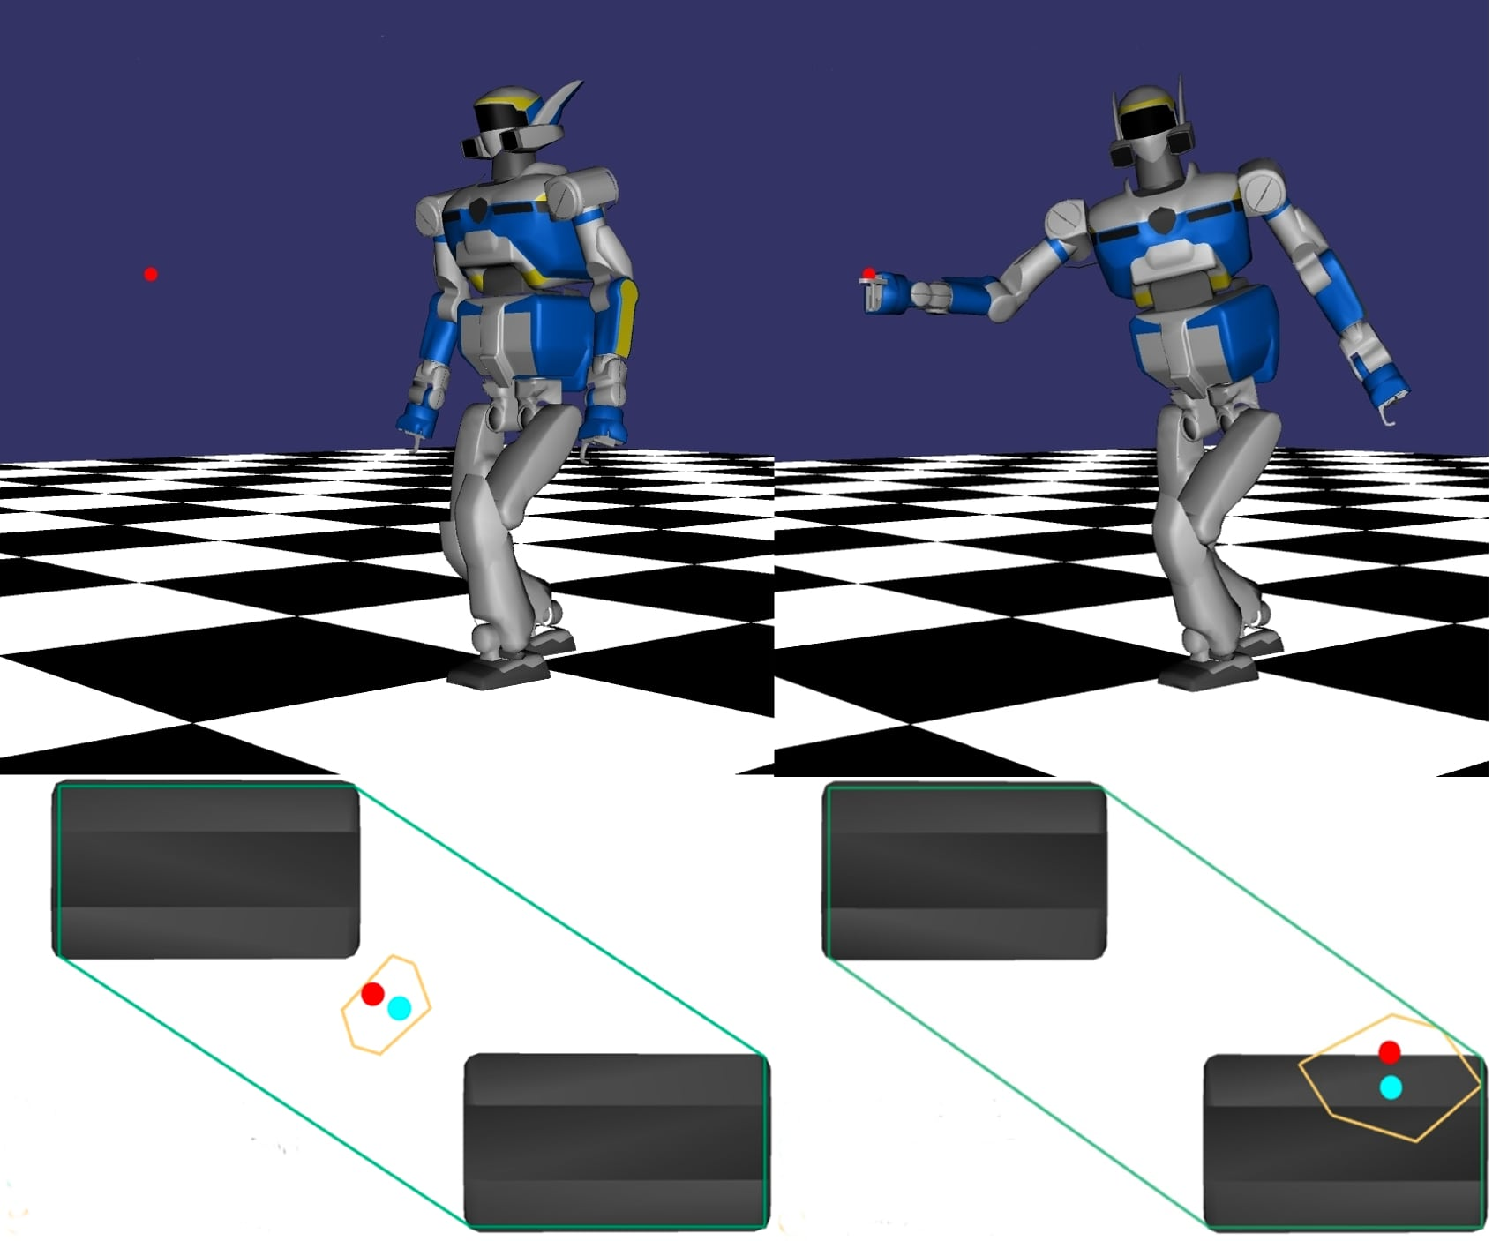
\includegraphics[scale=0.4]{rc_inertial_params/robust_merge.pdf}}\quad
\end{subfigure}\\
 \tikzcircle{3pt}  \footnotesize Real Capture Point \tikzcircle[turquoise, fill=turquoise]{3pt} Estimated Capture Point   \tikzcircle[green, fill=green]{3pt} Support Polygon   \tikzcircle[yellow, fill=yellow]{3pt} Capture Point Polytope

\caption{Screenshots of HRP-2 executing Test 1 to reach the ball target with the robust controller.}
\label{fig:control}
\end{figure*}


\begin{table*}[!tbph]
\begin{center}
\caption{Results of Test 1. For each controller we show the number of falls (Falls), the average time to complete the motion (Task Time) and the average distance of the end-effector to the target at the end of the motion (Task Error).}
\begin{tabular}{ |l|l|l|l|l|l|l|l| }
\hline
\multicolumn{2}{|c|}{Uncertainties}&\multicolumn{3}{|c|}{Classic Controller}&\multicolumn{3}{|c|}{Robust Controller}\\
\hline Max Mass & Max CoM &{Falls}& Task &{Task} & Falls & Task& Task  \\
Error & Error & & Time   &  Error & &  Time & Error\\ 
{[\%]} & [mm] & [\%]  &  [s]  &  [mm]  & [\%]  &  [s] & [mm]\\ 
\hline
% 10 & 12.5& 35& 6.22&4& 1& 5.26& 5\\
% 10 & 25  & 31 & 6.30&  5& 0& 7.32& 12\\
% 10 & 50  & 43 & 4.49 & 70 & 0 & 4.66 & 110\\
% 30 & 50  & 43 & 4.48 & 70 & 0 & 4.68 & 110\\
% 30 & 100 & 40 & 5.44 & 30 & 4 & 5.81 & 80 \\
10 & 10 & 31 & 4.4 & 49 & 3 & 4.5 & 60\\
10 & 20 & 33 & 4.3 & 52 & 1 & 4.5 & 69 \\
10 & 40 & 45 & 4.3 & 55 & 3 & 4.7 & 102\\ 
20 & 10 & 38 & 4.2 & 49 & 11 & 4.5 & 77\\
20 & 20 & 49 & 4.5 & 51 & 9 & 4.55 & 103 \\
20 & 40 & 45 & 4.5 & 59 & 14 & 4.72 & 122 \\
\hline
\end{tabular}
\label{tab:test1}
\end{center}
\end{table*}
\subsection{Test 1}
In this test we set the right end-effector target far in front of the robot.
Fig.~\ref{fig:control}  shows some screen shots of the simulations.
To reach the target the robot must move its CoM (and hence also its capture point) close to the boundaries of its support polygon. 
Table~\ref{tab:test1} presents the results. 
Regardless of the magnitude of the inertial parameter errors, the robust controller managed to prevent the robot from falling almost always, while with the  standard controller the robot fell more than 30\% of the times.
However, since the target was far away from the robot, the robust controller did not manage to reach it because that would have required violating the robust balance constraints.
\begin{table*}[!h]
\begin{center}
\caption{Results of Test 2. For each controller we show the number of falls (Falls), the average time to complete the motion (Task Time) and the average distance of the end-effector to the target at the end of the motion (Task Error).}
\begin{tabular}{ |l|l|l|l|l|l|l|l| }
\hline Max Mass & Max CoM &{Falls}& Task &{Task} & Falls & Task& Task  \\
Error & Error & & Time   &  Error & &  Time & Error\\ 
{[\%]} & [mm] & [\%]  &  [s]  &  [mm]  & [\%]  &  [s] & [mm]\\ 
\hline
% 10 & 12.5 & 59 & 3.64& 0 & 5 & 3.06& 0\\
% 10 & 25.0 & 42 & 3.40 & 0.18 & 4 & 2.94 & 0.12 \\
10 & 10 & 29 & 3.94 & 2 & 0 & 3.4 & 2 \\
10 & 20 & 35 & 3.4 & 2 & 2 & 3.0 & 2 \\
10 & 40 & 42 & 3.86 & 4 & 0 & 2.6 & 4 \\
20 & 10 & 43 & 3.6 & 3 & 0 & 2.8 & 4 \\
20 & 20 & 45 & 3.5 & 3 & 0 & 2.5 & 4 \\
20 & 40 & 45 & 3.0 & 5 & 0 & 2.1 & 5 \\

\hline
\end{tabular}
\label{tab:test2}
\end{center}
\end{table*}
\subsection{Test 2}
In this test we moved the right end-effector target closer to the robot, so that HRP-2 can reach it without moving its CoM close to the support polygon boundaries.
However, we increased the desired speed of reaching (by increasing the gains of the reaching task).
This affected the velocity of the CoM, which in turns affected the capture point, making it reach the boundaries of the support polygon.
The difference with respect to Test 1 is that in this case also the robust controller can reach the target.
Table~\ref{tab:test2} summarizes the results.

Similarly to Test 1, the classic controller leads the robot to a fall in more than 30\% of the cases.
However, contrary to Test 1, this time the robust controller also manages to reach the target, because it is located closer to the robot.
This test shows that being robust does not necessarily implies that we have to sacrifice performance.

